
\documentclass[twoside,12pt]{article}

\usepackage{dsctemplate}
\usepackage[margin=1in]{geometry}
\usepackage{amsmath}
\usepackage{amssymb,amsthm}
\usepackage{fancyhdr}
\usepackage{nicefrac}
\usepackage{minted}
\usetikzlibrary{quotes,angles,positioning,arrows.meta}
\usetikzlibrary{calc}
\usepackage{enumitem}
\usepackage{fancyvrb}
\usepackage{dirtytalk}
\usepackage{comment}
\usepackage{minted}

\DefineVerbatimEnvironment{verbatim}{Verbatim}{xleftmargin=.5in}
\newlist{multiplechoice}{itemize}{2}
\setlist[multiplechoice]{label=$\square$}

% configuration
% ------------------------------------------------------------------------------

% control whether solutions are shown or hidden
% \showsolntrue

% page headers only on odd pages
\pagestyle{fancy}
\fancyhead{}
\fancyhead[RO]{uniqname: \rule{3in}{.5pt}}
\renewcommand{\headrulewidth}{0pt}
% \pagenumbering{gobble}

% ------------------------------------------------------------------------------

\begin{document}


\thispagestyle{empty}

\vspace{-5.5in}

\pstitle{%
    Midterm Exam
}{EECS 398-003, Fall 2024}

\vspace{-.3in}

\begin{tabular}{rl}
    Full Name: & \inlineresponsebox[4in]{Solutions}\\
    Uniqname: & \inlineresponsebox[4in]{rampure}\\
    UMID: & \inlineresponsebox[4in]{12345678} \vspace{0.2in} \\
    Room: & \bubble{CHRYS 133} \bubble{IOE 1610} \bubble{IOE 1680} \bubble{COOL 1940} \vspace{.3in} \\ 
\end{tabular}

\vspace{.1in}

\hline

\vspace{.1in}


\textbf{Instructions:}
    \begin{itemize}
       \item This exam consists of 14 questions, worth a total of 100 points. You have 120 minutes to complete the exam.
        \item Write your uniqname in the top right corner of each page in the space provided.
        \item Please write \textbf{clearly} in the provided answer boxes; we will not grade work that appears elsewhere. Completely fill in bubbles and square boxes; if we cannot tell which option(s) you selected, you may lose points.
        
            \bubble{A bubble means that you should only \textbf{select one choice}.}
            
            \squarebubble{A square box means you should \textbf{select all that apply}.}
            
        \item You may refer to a single two-sided handwritten notes sheet. Other than that, you may not refer to any other resources or technology during the exam (no phones, watches, or calculators).
    \end{itemize}

\vspace{.1in}

\hline

\vspace{0.1in}

\noindent You are to abide by the University of Michigan/Engineering Honor Code. To receive a grade,
please sign below to signify that you have kept the honor code pledge.

\vspace{0.2in}

\noindent \textit{I have neither given nor received aid on this exam, nor have I concealed any violations of the
Honor Code.}

\vspace{0.2in}

\begin{tabular}{rl}
    \: \: \: \: \: Signature: & \biginlineresponsebox[4in]{}\\
\end{tabular}

\begin{center}

\vspace{0.3in}

\huge{Version A}

\end{center}

\newpage

\begin{center}
    \noindent \textbf{\large{Data Overview: Flight Reviews}} 
\end{center}

\noindent Skytrax is a website that allows anyone to submit a review for a flight they took. In this exam, we'll work with the DataFrame \texttt{reviews}, which contains flight reviews taken from Skytrax.

\vspace{.1in}

\noindent The first few rows of \texttt{reviews} are shown below, but \texttt{reviews} has many more rows than are shown.

% \vspace{-.5in}

\begin{center}

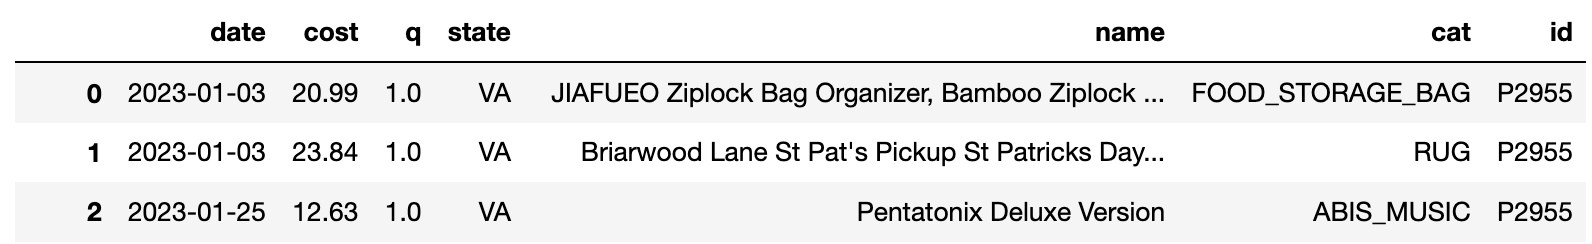
\includegraphics[width=\textwidth]{midterm-images/df.png}

\end{center}

\vspace{.1in}

\noindent The columns in \texttt{reviews} are as follows:

\begin{itemize}

\item{\texttt{"airline" (str)}: The airline flown. Note that an airline can be reviewed multiple times.}
\item \texttt{"author" (str)}: The author of the review. Note that an author can write multiple reviews (and can even write multiple reviews of the same airline!).
\item \texttt{"date" (str)}: The date on which the review was written. Most of the reviews were written in 2015.
\item \texttt{"content" (str)}: The content of the review.
\item \texttt{"cabin" (str)}: The cabin the author flew; either \texttt{"Economy"}, \texttt{"Premium Economy"}, \texttt{"Business"}, or \texttt{"First"}.
\item \texttt{"overall" (int)}: The overall rating the author gave their flight experience, between 0 and 10 (inclusive).

\end{itemize}


\noindent \textbf{Throughout the exam}, assume we have already run \texttt{import pandas as pd} and \texttt{import numpy as np}.

\newpage

\noindent \textbf{Make sure you have read the Data Overview before beginning!}

\begin{probset}

\begin{prob}[(6 pts)]
Fill in the blanks so that \texttt{santas\_airlines} evaluates to an array containing the \textbf{unique} names of the airlines that Santa Ono has reviewed.

\begin{verbatim}
santas_airlines = reviews.loc[__(i)__, __(ii)__].__(iii)__
\end{verbatim}

\begin{tabular}{ll}
\texttt{(i)}: & \inlineresponsebox[5.68in]{}\\
\texttt{(ii)}: & \inlineresponsebox[2.5in]{} \texttt{(iii)}: \inlineresponsebox[2.5in]{}\\
\end{tabular}
    
\end{prob}

\begin{prob}[(6 pts)]

Consider the function \texttt{operate}, defined below.

\begin{verbatim}
def operate(df):
    df["content"] = df["content"].str.split().str.len()
\end{verbatim}

Consider the following six answer choices:

\begin{enumerate}[label=\Alph*.]

\item{Nothing, because we didn't reassign \texttt{reviews} after calling \texttt{operate(reviews)}.}

\item{\texttt{reviews["content"]} now contains the number of characters per review.}

\item{\texttt{reviews["content"]} now contains the number of words per review.}

\item{We see an error because we're trying to use \texttt{.str} methods on an invalid column.}

\item{We see an error because a column with the name \texttt{"content"} already exists.}

\item{We see an error because we're assuming \texttt{df} is a DataFrame but it is \texttt{None} (null).}
\end{enumerate}

All three parts of this question are \textbf{independent} from one another; the code in earlier parts should not influence your answers in later parts. 

\begin{subprobset}

\begin{subprob}(2 pts) What happens after running the following block of code?

\begin{verbatim}
operate(reviews)
\end{verbatim}

\bubble{A} 
\bubble{B} 
\bubble{C} 
\bubble{D} 
\bubble{E} 
\bubble{F}

\end{subprob}

\vspace{.1in}

\begin{subprob}(2 pts) What happens after running the following block of code?

\begin{verbatim}
operate(reviews)
operate(reviews)
\end{verbatim}

\bubble{A} 
\bubble{B} 
\bubble{C} 
\bubble{D} 
\bubble{E} 
\bubble{F}

\end{subprob}

\vspace{.1in}

\begin{subprob}(2 pts) What happens after running the following block of code?

\begin{verbatim}
reviews = operate(reviews)
reviews = operate(reviews)
\end{verbatim}

\bubble{A} 
\bubble{B} 
\bubble{C} 
\bubble{D} 
\bubble{E} 
\bubble{F}

\end{subprob}
    
\end{subprobset}
    
\end{prob}

\newpage

\begin{prob}[(8 pts)]

Suppose we define \texttt{n = reviews.shape[0]}.

% Suppose we define \texttt{n} as follows:

% \begin{verbatim}
%     n = reviews.shape[0]
% \end{verbatim}

In each of the four parts of this question, we provide an expression that evaluates to a new DataFrame. Depending on the expression, the new DataFrame:
\begin{itemize}
    \item May or may not have the same number of rows as \texttt{reviews}.
    \item May have some rows from \texttt{reviews} appear multiple times (i.e. may have duplicated rows). Note that \texttt{reviews} itself \textbf{does not} have any duplicated rows.
    \item May have rows that appear in a different order than they appeared in \texttt{reviews}.
\end{itemize}

For example, if \texttt{df} is on the left, the DataFrame on the right has the same number of rows as \texttt{df}, has some duplicated rows (row 1 appears twice), and has the same row order as \texttt{df} (all row 0s before row 1s, all row 1s before row 2s, etc.).

\begin{center}

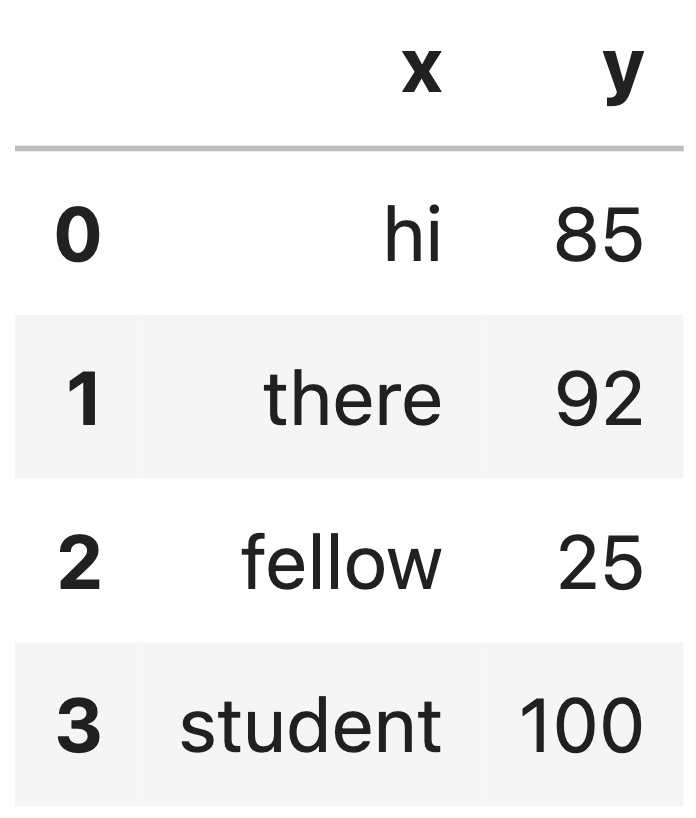
\includegraphics[width=0.17\textwidth]{midterm-images/df-1.png} \hspace{0.5in} 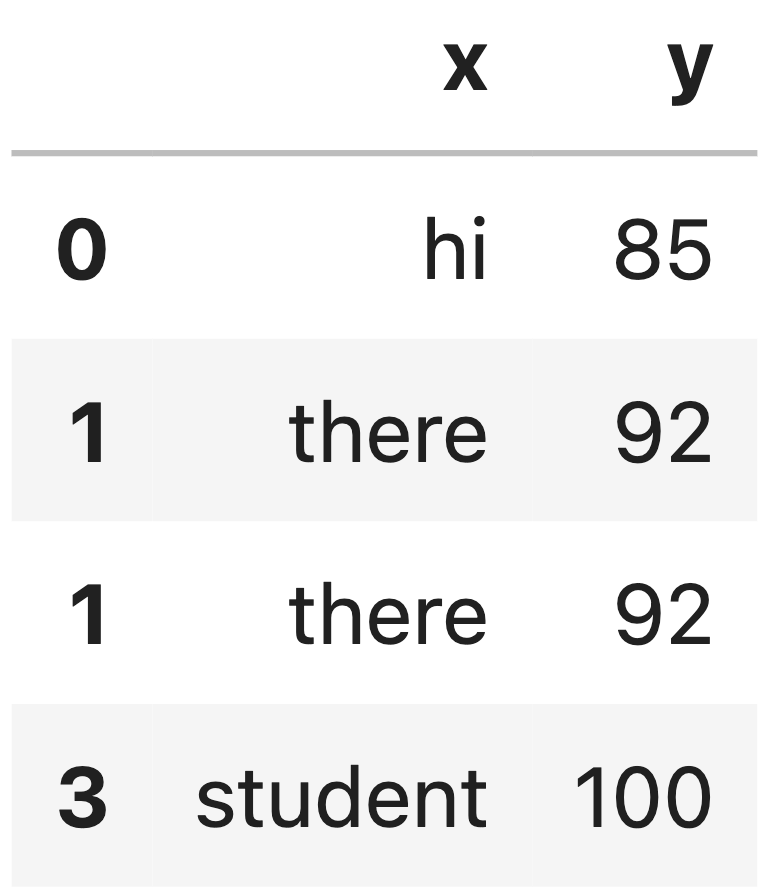
\includegraphics[width=0.17\textwidth]{midterm-images/df-2.png}
    
\end{center}

Select the options that correctly describe the DataFrame that results from each of the following expressions.

\begin{subprobset}

\begin{subprob}(2 pts) \hspace{0.1in} \texttt{reviews.loc[np.random.choice([True, False], size=n, replace=True)]}

% What does the following block of code evaluate to?

% \begin{verbatim}

% \end{verbatim}

\begin{tabular}{lllll}
(i) & Same number of rows as \texttt{reviews}? & \bubble{Yes} &  \bubble{No} \\
(ii) & Possibility of duplicated rows? & \bubble{Yes} & \bubble{No} \\
(iii) & Row order guaranteed to be the same as \texttt{reviews}? & \bubble{Yes} & \bubble{No}
\end{tabular}

\end{subprob}

\begin{subprob}(2 pts) \hspace{0.1in} \texttt{reviews.loc[np.random.permutation(np.arange(n))]}

\begin{tabular}{lllll}
(i) & Same number of rows as \texttt{reviews}? & \bubble{Yes} &  \bubble{No} \\
(ii) & Possibility of duplicated rows? & \bubble{Yes} & \bubble{No} \\
(iii) & Row order guaranteed to be the same as \texttt{reviews}? & \bubble{Yes} & \bubble{No}
\end{tabular}
    
\end{subprob}    

\begin{subprob}(2 pts) \hspace{0.1in} \texttt{reviews.loc[np.random.choice(np.arange(n), size=n, replace=True)]}

\begin{tabular}{lllll}
(i) & Same number of rows as \texttt{reviews}? & \bubble{Yes} &  \bubble{No} \\
(ii) & Possibility of duplicated rows? & \bubble{Yes} & \bubble{No} \\
(iii) & Row order guaranteed to be the same as \texttt{reviews}? & \bubble{Yes} & \bubble{No}
\end{tabular}
    
\end{subprob}

\begin{subprob}(2 pts) \hspace{0.1in} \texttt{reviews.loc[np.random.choice(np.arange(n), size=n, replace=False)]}

\begin{tabular}{lllll}
(i) & Same number of rows as \texttt{reviews}? & \bubble{Yes} &  \bubble{No} \\
(ii) & Possibility of duplicated rows? & \bubble{Yes} & \bubble{No} \\
(iii) & Row order guaranteed to be the same as \texttt{reviews}? & \bubble{Yes} & \bubble{No}
\end{tabular}
    
\end{subprob}

\end{subprobset}
    
\end{prob}

\newpage

\begin{prob}[(8 pts)]

The bar chart below shows the distribution of the number of reviews per \texttt{"author"} in \texttt{reviews}. For instance, it's telling us that approximately 120 \texttt{"author"}s wrote 2 reviews. \textbf{Assume that the height of the bar at 8 on the $x$-axis is exactly 1, and that this is the shortest bar (with no ties).}
\vspace{-0.1in}
\begin{center}
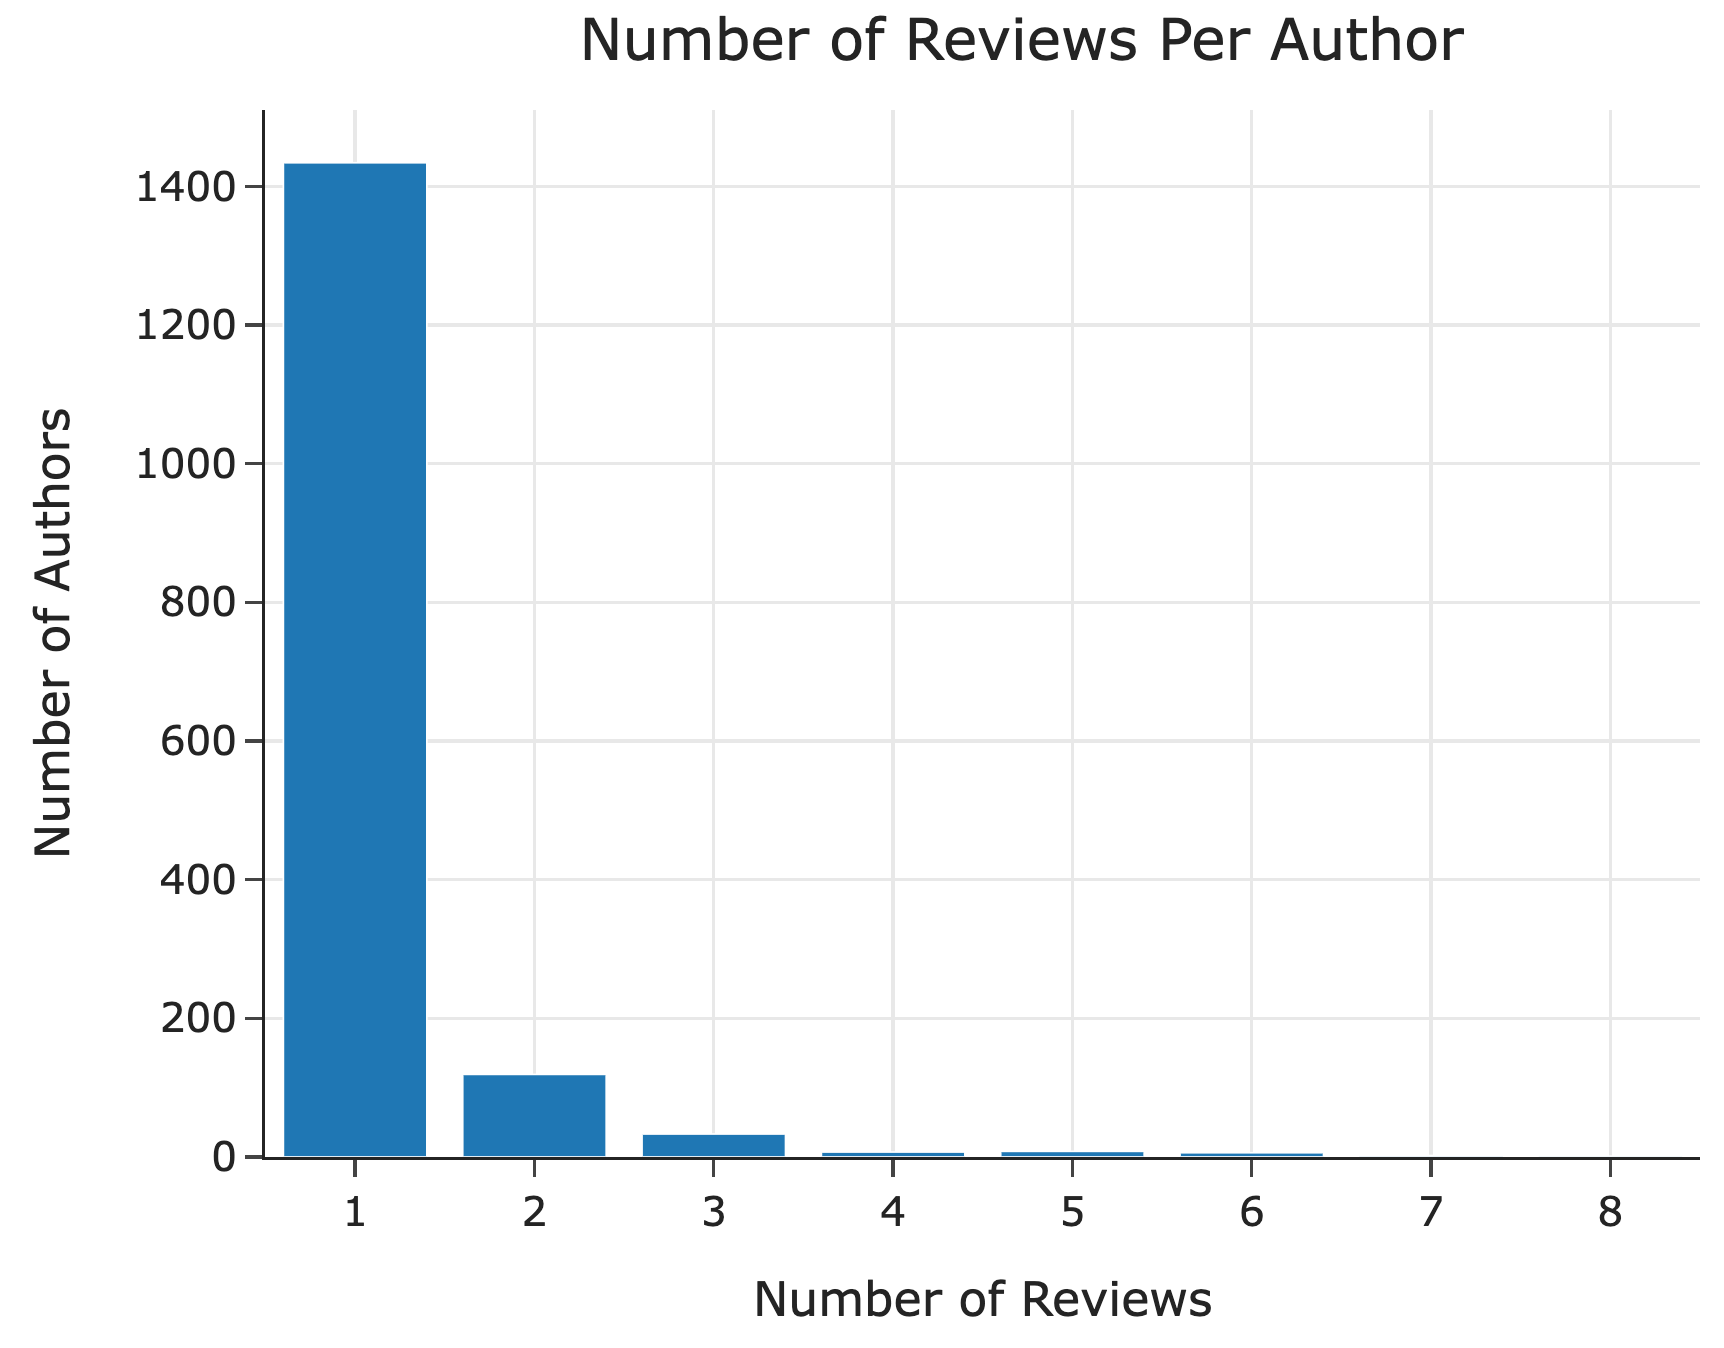
\includegraphics[width=0.5\textwidth]{midterm-images/reviews-per-author.png}
\end{center}
\vspace{-0.2in}

Hint: The \textbf{values} in the Series that results from calling \texttt{value\_counts()} are sorted in descending order.

\begin{subprobset}

\begin{subprob}(2 pts) Fill in the blank below so that \texttt{W} evaluates to the value \texttt{7}.

\begin{verbatim}
W = reviews["author"].value_counts().__(i)__
\end{verbatim}

\texttt{(i)}: \hspace{0.01in} \inlineresponsebox[4in]{}
    
\end{subprob}
    
\end{subprobset}

Now, consider the values defined below. \vspace{-0.1in}

\begin{verbatim}
W = reviews["author"].value_counts().value_counts().loc[1]
X = reviews["author"].value_counts().value_counts().iloc[1]
Y = reviews["author"].value_counts().value_counts().index[1]
Z = reviews["author"].value_counts().value_counts().index[-1]
\end{verbatim}

\begin{subprobset}

\begin{subprob}(2 pts) Which value is equal to \textbf{8}?

\bubble{\texttt{W}}
\bubble{\texttt{X}}
\bubble{\texttt{Y}}
\bubble{\texttt{Z}}
\bubble{None of these.}

\end{subprob}

\begin{subprob}(2 pts) Which value is equal to \textbf{the height of the tallest bar}?

\bubble{\texttt{W}}
\bubble{\texttt{X}}
\bubble{\texttt{Y}}
\bubble{\texttt{Z}}
\bubble{None of these.}

\end{subprob}

\begin{subprob}(2 pts) Which value is equal to \textbf{the height of the second-tallest bar}?

\bubble{\texttt{W}}
\bubble{\texttt{X}}
\bubble{\texttt{Y}}
\bubble{\texttt{Z}}
\bubble{None of these.}

\end{subprob}
    
\end{subprobset}
    
\end{prob}

\newpage

\begin{prob}[(4 pts)]
\textbf{Select all} visualization techniques we \textit{could} use to visualize the distribution of \texttt{"overall"} ratings, separately for Delta Air Lines and United Airlines. At least one answer is correct.

\squarebubble{side-by-side box plots}

\squarebubble{side-by-side bar charts}

\squarebubble{a scatter plot}

\squarebubble{a pie chart}

\squarebubble{overlaid histograms}
    
\end{prob}

\begin{prob}[(8 pts)]

We define the \textbf{robust mean} of a collection of values to be the mean of all values, once the largest and smallest values are removed. For example, the robust mean of $2, 2, 3, 7, 12$ is $\frac{2+3+7}{3} = 4$.

In part (a), fill in the blanks so that \texttt{worst\_robustly} evaluates to the \texttt{"airline"} with the lowest robust mean of \texttt{"overall"} ratings. Assume there are no ties in robust ratings, and that each \texttt{"airline"} has at least 3 ratings.

\begin{verbatim}
def funky(x):
    return __(iii)__

worst_robustly = reviews.__(i)__["overall"].__(ii)__(funky).idxmin()
\end{verbatim}

\begin{subprobset}

\begin{subprob}(6 pts)

\texttt{(i)}: \hspace{0.02in} \begin{tabular}{ll}
\bubble{\texttt{sort\_values("overall")}} & \bubble{\texttt{sort\_values("airline")}} \\
\bubble{\texttt{groupby("overall")}} & \bubble{\texttt{groupby("airline")}} \\
\bubble{\texttt{value\_counts("overall")}} & \bubble{\texttt{value\_counts("airline")}}
\end{tabular}

\vspace{0.2in}

\texttt{(ii)}: \hspace{0.0in} 

\bubble{\texttt{agg}} 
\bubble{\texttt{filter}}
\bubble{\texttt{transform}}

\vspace{0.2in}

\texttt{(iii)}: \biginlineresponsebox[6in]{}
    
\end{subprob}

\begin{subprob}(2 pts) What are the input and output types of the function \texttt{funky}?

\bubble{Input: Series, Output: Number} 

\bubble{Input: Series, Output: Series}

\bubble{Input: Series, Output: DataFrame}

\bubble{Input: DataFrame, Output: Number} 

\bubble{Input: DataFrame, Output: Series}

\bubble{Input: DataFrame, Output: DataFrame}
    
\end{subprob}
    
\end{subprobset}

\vspace{0.2in}

\end{prob}

\newpage

\begin{prob}[(9 pts)]

Consider the DataFrame \texttt{imp}, shown in its entirety below.

\begin{center}
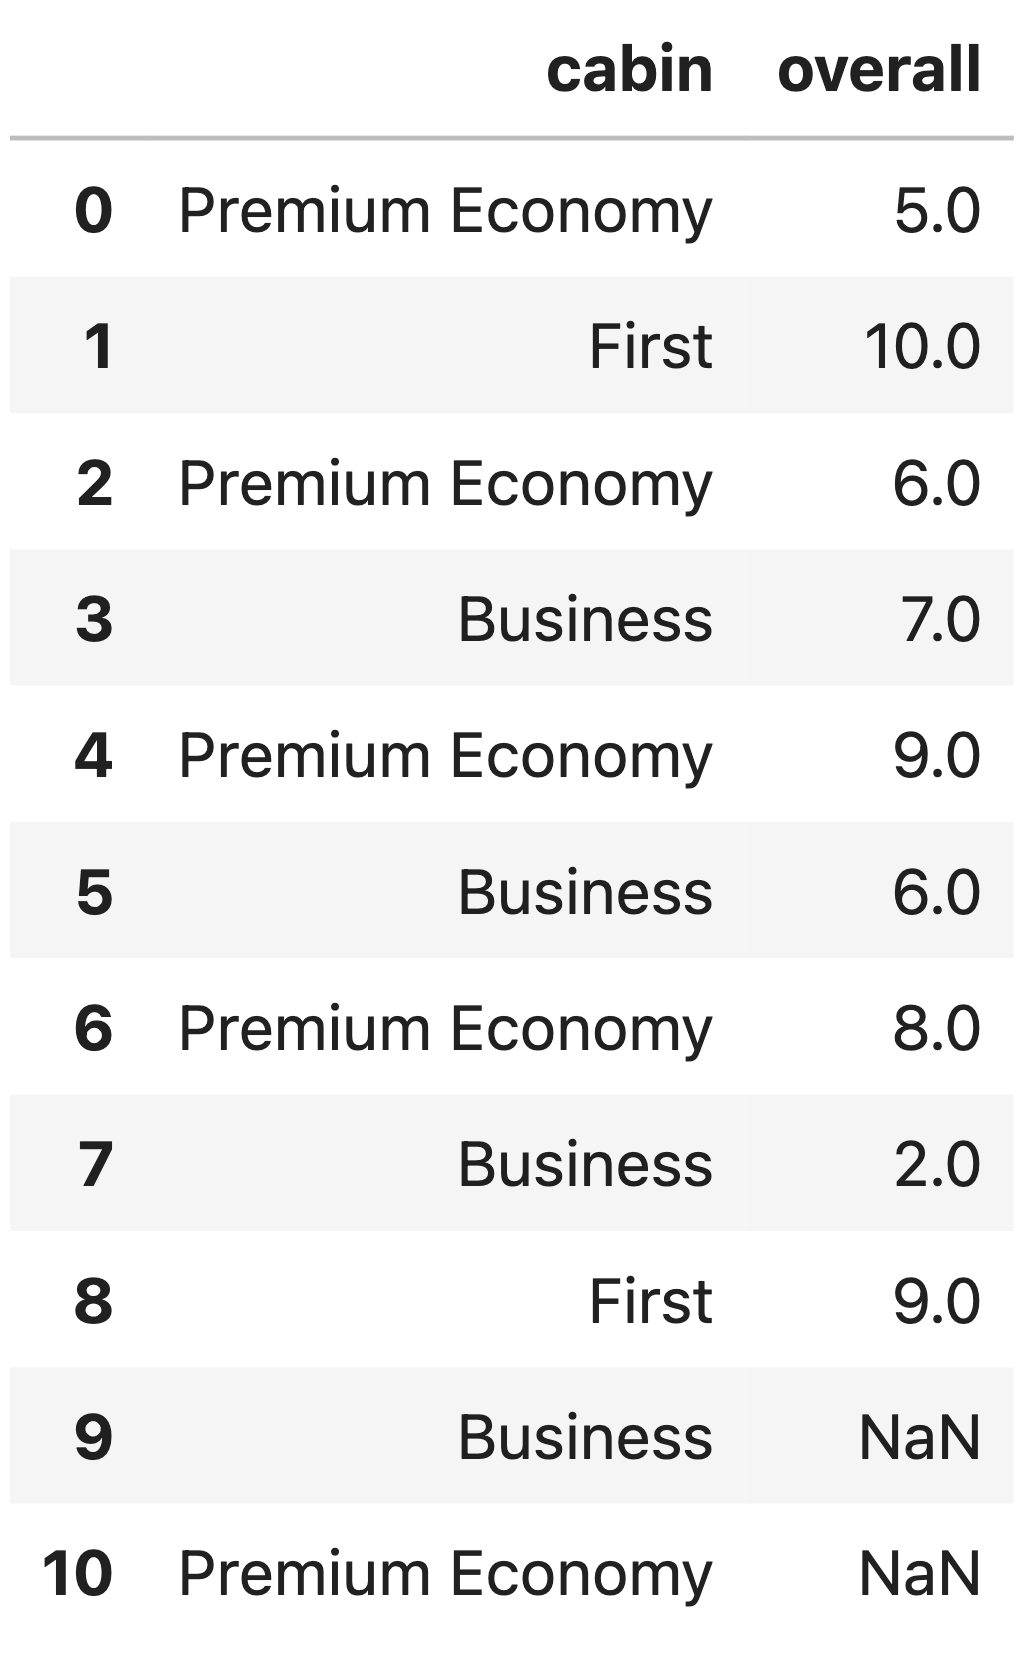
\includegraphics[width=0.35\textwidth]{midterm-images/imp.png}
\end{center}

As in the previous question, we define the \textbf{robust mean} of a collection of values to be the mean of all values, once the largest and smallest values are removed. For example, the robust mean of $2, 2, 3, 7, 12$ is $\frac{2+3+7}{3} = 4$.

\begin{subprobset}

\begin{subprob}(6 pts) Suppose we use \textbf{robust mean imputation, conditional on \texttt{"cabin"}} to fill in the missing values in the \texttt{"overall"} column. In  doing so, what are the missing values in the \texttt{"overall"} column filled in with? Give your answers as \textbf{numbers}.

Missing value in row \texttt{9}: \inlineresponsebox[1in]{} \hspace{in} Missing value in row \texttt{10}: \inlineresponsebox[1in]{}
    
\end{subprob}

\begin{subprob}(3 pts) Suppose \texttt{imp} represents the DataFrame above, with 2 missing values, and \texttt{filled} represents the DataFrame that results from imputing the missing values in \texttt{imp} in the way described in the previous part. In the following code block, what is the value of \texttt{comp}?

\begin{verbatim}
old_means = imp.groupby("cabin")["overall"].mean()
comp = old_means == filled.groupby("cabin")["overall"].mean()
\end{verbatim}

\begin{tabular}{lll}
\bubble{\texttt{True}} & \bubble{\texttt{False}} \\
\bubble{The Series \texttt{[True, True, True]}} & \bubble{The Series \texttt{[False, False, False]}} \\
\bubble{The Series \texttt{[True, True, False]}} & \bubble{The Series \texttt{[True, False, True]}} \\
\bubble{The Series \texttt{[False, True, True]}} & \bubble{The Series \texttt{[False, False, True]}} \\
\bubble{The Series \texttt{[False, True, False]}} & \bubble{The Series \texttt{[True, False, False]}} \\


% \\ \bubble{The Series \texttt{[False, True, False]}} & \bubble{The Series \texttt{[True, False, True]}}
% \\ \bubble{The Series \texttt{[False, False, True]}} & \bubble{The Series \texttt{[True, True, False]}}

\end{tabular}

\small{Hint: When grouping, the index is automatically sorted in ascending order.}
    
\end{subprob}
    
\end{subprobset}
    
\end{prob}

\newpage

\begin{prob}[(8 pts)]

Consider the DataFrame \texttt{framer}, defined below.
\begin{verbatim}
framer = reviews.pivot_table(index="airline",
                             columns="cabin",
                             values="author",
                             aggfunc="max")
\end{verbatim}

\begin{subprobset}

\begin{subprob}(3 pts) In one English sentence, describe the meaning of the \textbf{value} that the following expression evaluates to.

\begin{verbatim}
framer.loc["emirates", "Economy"]
\end{verbatim}

\begin{responsebox}{1in}
The last name, alphabetically, among all authors who submitted an Economy Class Emirates review.
\end{responsebox}
    
\end{subprob}

\begin{subprob}(2 pts) What is the value of the following expression?

\begin{verbatim}
framer.isna().sum(axis=0).shape[0]
\end{verbatim}

\bubble{The number of unique values in the \texttt{"airline"} column of \texttt{reviews}.}

\bubble{The number of unique values in the \texttt{"cabin"} column of \texttt{reviews}.}

\bubble{The number of unique values in the \texttt{"author"} column of \texttt{reviews}.}

\bubble{The number of unique values in the \texttt{"overall"} column of \texttt{reviews}.}

\bubble{None of the above.}

\end{subprob}

\begin{subprob}(3 pts) Consider the following information.

\begin{verbatim}
>>> framer.isna().sum(axis=0).sum()
320
>>> reviews["airline"].nunique()
125
>>> reviews["cabin"].nunique()
4
\end{verbatim} 

What is the value of the following expression? Show your work, and $\boxed{\text{box}}$ your final answer, which should be a \textbf{positive integer}.

\begin{verbatim}
reviews.groupby(["airline", "cabin"])["overall"].mean().shape[0]
\end{verbatim}

\biginlineresponsebox[6in]{}

\end{subprob}
    
\end{subprobset}
    
\end{prob}

\newpage

\begin{prob}[(10 pts)]

Consider the DataFrame \texttt{lines}, created by keeping the rows in \texttt{reviews} corresponding to reviews written between 2015-11-24 and 2015-11-28. Remember, each row in \texttt{lines} corresponds to a review of an \textbf{airline}.

Also consider the DataFrame \texttt{ports}, in which each row corresponds to a review of a particular \textbf{airport}. \texttt{ports} has a \texttt{"date"} column, too, and also only has reviews written between 2015-11-24 and 2015-11-28.

Consider the following information.

\vspace{0.1in}

\hline

\vspace{-0.1in}

\begin{verbatim}
>>> lines["date"].value_counts().sort_index()
2015-11-24      2
2015-11-25      7
2015-11-26      1
2015-11-27      4
>>> ports.shape[0]
17
>>> ports["date"].unique()
array(["2015-11-26", "2015-11-27", "2015-11-28"])
>>> lines.merge(ports, on="date", how="inner").shape[0]
29
>>> lines.merge(ports, on="date", how="outer").shape[0]
41
\end{verbatim}

\hline

\vspace{0.1in}

Below, give your answers as \textbf{integers}.
\begin{subprobset}
\begin{subprob}(2 pts) How many values in \texttt{ports["date"]} are equal to \texttt{"2015-11-24"}? \inlineresponsebox[1.25in]{}
\end{subprob}

\begin{subprob}(2 pts) How many values in \texttt{ports["date"]} are equal to \texttt{"2015-11-25"}? \inlineresponsebox[1.25in]{}
\end{subprob}

\begin{subprob}(2 pts) How many values in \texttt{ports["date"]} are equal to \texttt{"2015-11-26"}? \inlineresponsebox[1.25in]{}
\end{subprob}

\begin{subprob}(2 pts) How many values in \texttt{ports["date"]} are equal to \texttt{"2015-11-27"}? \inlineresponsebox[1.25in]{}
\end{subprob}

\begin{subprob}(2 pts) How many values in \texttt{ports["date"]} are equal to \texttt{"2015-11-28"}? \inlineresponsebox[1.25in]{}
\end{subprob}

\end{subprobset}

\newpage

\begin{prob}[(4 pts)]
    % Neeru urgently needs to return to Ann Arbor from the United Kingdom because his AWS Lambda instance is stuck in an infinite loop! However, he will only consider certain airlines. Provided below is a SQL query that correctly finds all valid airlines according to his specifications. Choose the correct pandas implementation that emulates the behavior of this query. 

Consider the following SQL query.

\begin{verbatim}
SELECT author, AVG(overall) AS average_overall FROM reviews
GROUP BY author
HAVING AVG(overall) >= 8 AND COUNT(*) >= 5
ORDER BY average_overall;
\end{verbatim}

Now, consider the following four code blocks.

\begin{itemize}
    \item Block 1:
\begin{verbatim}
f = lambda x: x["overall"].mean() >= 8 and x.shape[0] >= 5
pop_auth = (reviews.groupby("author").filter(f)
                   .groupby("author")[["overall"]].mean()
                   .sort_values("overall").reset_index())
\end{verbatim}

    \item Block 2:
\begin{verbatim}
g = lambda x: x.shape[0] >= 5
pop_auth = (reviews[reviews["overall"] >= 8]
            .groupby("author").filter(g)
            .groupby("author")[["overall"]].mean()
            .sort_values("overall").reset_index())
\end{verbatim}
    \item Block 3:
\begin{verbatim}
pop_auth = (reviews["author"].value_counts().reset_index()
            .merge(
                reviews.groupby("author")[["overall"]].mean().reset_index(), 
                on="author")
            .pipe(lambda x: x[(x["overall"] >= 8)])
            .sort_values("overall")
            .pipe(lambda r: r[r["count"] >= 5])
            [["author", "overall"]])
\end{verbatim}

    \item Block 4:
\begin{verbatim}
temp = reviews.groupby("author")["overall"].agg(["count", "mean"])
pop_auth = (temp[(temp["count"] >= 5) & (temp["mean"] >= 8)]
            .sort_values("mean")
            .reset_index()[["author", "mean"]])
\end{verbatim}

\end{itemize}

Three of the blocks above correctly assign \texttt{pop\_auth} to a DataFrame that is equivalent to the table outputted by the SQL query at the top of the page (ignoring the names of the resulting columns and the values in the index). One of the options \textbf{is incorrect}.

Which block is \textbf{incorrect} --- that is, which block \textbf{does not} assign \texttt{pop\_auth} so that it is equivalent to the result of the SQL query at the top of the page?

\bubble{Block 1}
\bubble{Block 2}
\bubble{Block 3}
\bubble{Block 4}


%     \bubble{a} 
%     \begin{verbatim}
%     df.groupby("airline_name").agg(
%         avg_rating=("overall_rating", "mean"),
%         avg_food_rating=("food_beverages_rating", "mean"),
%         avg_seat_comfort=("seat_comfort_rating", "mean")
%     ).apply(lambda x: x["avg_food_rating"] + x["avg_seat_comfort"] > 7.0 
%     and x["avg_rating"] >= 6.0)
%     \end{verbatim}
%     % We us apply incorrectly in this example
%     \bubble{b}
%     \begin{verbatim}
%     grouped = df.groupby("airline_name").agg(
%     avg_rating=("overall_rating", "mean"),
%     avg_food_rating=("food_beverages_rating", "mean"),
%     avg_seat_comfort=("seat_comfort_rating", "mean")
%     )
%     grouped[grouped["avg_rating"] >= 6.0]
%     \end{verbatim}
%     % We ignore the other 2 filters, avg food rating and avg seat comfort being greater than 7.0
%     \bubble{c}
%     \begin{verbatim}
%     grouped = df.groupby("airline_name").agg(
%     avg_rating=("overall_rating", "mean"),
%     avg_food_rating=("food_beverages_rating", "mean"),
%     avg_seat_comfort=("seat_comfort_rating", "mean")
%     )
%     grouped[(grouped["avg_rating"] >= 6.0) & 
%         (grouped["avg_food_rating"] + grouped["avg_seat_comfort"] > 7.0)]
% \end{verbatim}
%      % correct

%     \bubble{d}
%     \begin{verbatim}
%     df.groupby("airline_name").agg(
%     avg_rating=("overall_rating", "mean"),
%     total_score=("food_beverages_rating", "sum") + ("seat_comfort_rating", "sum")
%     ).loc[lambda x: x["avg_rating"] >= 6.0]
% \end{verbatim}
%     % This one incorrectly calulates total score, should sum the averages not the individual sums

\end{prob}

\newpage

\begin{prob}[(8 pts)]

Suppose we define \texttt{soup} to be a BeautifulSoup object that is instantiated using the HTML document below. (To save space, we've omitted the tags \texttt{<html>} and \texttt{</html>}.)
\begin{verbatim}
<title>Aalborg Airport Customer Reviews - SKYTRAX</title>
<a href="https://www.airlinequality.com" rel="nofollow">
    <img src="https://www.airlinequality.com/images/skytrax.svg" alt="SKYTRAX">
</a>
<div class="skytrax-ratings">
    <table class="review-ratings">
        <tr>
            <td class="terminal-cleanliness">Terminal Cleanliness</td>
            <td>4</td>
        </tr>
        <tr>
            <td class="food-beverages">Food Beverages</td>
            <td>9</td>
        </tr>
        <tr>
            <td class="airport-staff">SKYTRAX Staff</td>
            <td>3</td>
        </tr>
    </table>
</div>
\end{verbatim}

In parts (a) and (b), fill in the blanks so that each expression evaluates to \texttt{"SKYTRAX"}.

\begin{subprobset}

\begin{subprob}(2 pts) \hspace{0.1in} \verb|soup.__(i)__("alt")|

\texttt{(i)}: \hspace{0.01in} \inlineresponsebox[4in]{}
    
\end{subprob}

\begin{subprob}(3 pts) \hspace{0.1in} \verb|soup.find("td", __(i)__).text.__(ii)__|

\texttt{(i)}: \hspace{0.01in} \inlineresponsebox[4in]{}

\texttt{(ii)}: \inlineresponsebox[4in]{}
    
\end{subprob}

\newpage

\begin{subprob}(3 pts) Fill in the blanks so that \texttt{avg\_rating} evaluates to the mean of the three ratings in the document above. (In the document, the three ratings are 4, 9, and 3, but you \textbf{shouldn't} hard-code these values.)

\begin{verbatim}
texts = [tag.text for tag in soup.find_all("td")]
avg_rating = np.mean([__(i)__ for j in range(__(ii)__)])
\end{verbatim}

\texttt{(i)}: \hspace{0.01in} \inlineresponsebox[4in]{}

\texttt{(ii)}: \inlineresponsebox[4in]{}
    
\end{subprob}

% \begin{subprob}

% \begin{verbatim}
% soup.find("td", __(i)__).text.__(ii)__
% \end{verbatim}

% \texttt{(i)}: \inlineresponsebox[2.5in]{} \texttt{(ii)}: \inlineresponsebox[2.5in]{}
    
% \end{subprob}

\end{subprobset}
    
% \end{prob}
    
\end{prob}

\vspace{0.4in }

\begin{prob}[(4 pts)] 

All airports have IATA codes, which are strings of three uppercase letters that uniquely identify the airport. For example, Detroit's IATA code is \texttt{"DTW"}. Many of the entries in the \texttt{"content"} column of \texttt{reviews} use IATA codes to describe the route flown.

We define a \textbf{route string} as being a pair of IATA codes separated by \texttt{"-"} or \texttt{" to "} (pay close attention to the spacing). For example, in \texttt{test\_review} there are two route strings, \texttt{"YWG-LHR"} and \texttt{"EDI to YWG"}:

\begin{verbatim}
test_review = """I recently traveled YWG-LHR and returned home from 
                 EDI to YWG with AC Rouge. I must say I was
                 pleasantly surprised with how well the trip went
                 in both directions, but I'm glad I didn't have to
                 transit in ORD."""
\end{verbatim}

Fill in the blank below with a regular expression that matches valid route strings.

\begin{center}
\texttt{" }\biginlineresponsebox[6in]{} \texttt{"}
\end{center}
    
\end{prob}


\newpage

\begin{prob}[(8 pts)]

Consider the string \texttt{thoughts}, defined below:

\begin{verbatim}
thoughts = """Brought my Sony A5000 for my trip
              the Airbus A220v300's bathroom has a window
              My favorite jet is the B737-900ER flew it like x 239
              all stan the queen B747, 120% the B333st
              I like the chonky A380
              but I love the A350"""
\end{verbatim}

There are exactly 5 valid \textbf{plane codes} in \texttt{thoughts}: \texttt{"A220"}, \texttt{"B737"}, \texttt{"B747"}, \texttt{"A380"}, and \texttt{"A350"}. For each regular expression \texttt{exp} below,
\begin{itemize}
    \item specify the number of valid plane codes that the expression \texttt{re.findall(exp, thoughts)} extracts in their entirety, and
    \item specify the number of \textbf{other, invalid} strings that \texttt{re.findall(exp, thoughts)} also extracts.
\end{itemize}
The first example has been done for you.

\begin{subprobset}

\begin{subprob} \verb|exp = r"B\d{3}"|

Valid plane codes extracted: \boxedinlineresponsebox[1in]{2} \hspace{0.3in} Invalid strings extracted: \boxedinlineresponsebox[1in]{1}
    
\end{subprob}
\vspace{0.2in}

\begin{subprob}(2 pts) \verb|exp = r"[AB]\d{3}"|

Valid plane codes extracted: \inlineresponsebox[1in]{5} \hspace{0.3in} Invalid strings extracted: \inlineresponsebox[1in]{2}
    
\end{subprob}
\vspace{0.2in}

\begin{subprob}(2 pts) \verb!exp = r"A\d{2}0|B7\d7"!

Valid plane codes extracted: \inlineresponsebox[1in]{5} \hspace{0.3in} Invalid strings extracted: \inlineresponsebox[1in]{1}
    
    
\end{subprob}
\vspace{0.2in}

\begin{subprob}(2 pts) \verb!exp = r"A[23]\d0|B7\d7"!

Valid plane codes extracted: \inlineresponsebox[1in]{5} \hspace{0.3in} Invalid strings extracted: \inlineresponsebox[1in]{0}
    
\end{subprob}
\vspace{0.2in}

\begin{subprob}(2 pts) \verb!exp = r"(A[23]\d0|B7\d7)$"!

Valid plane codes extracted: \inlineresponsebox[1in]{2} \hspace{0.3in} Invalid strings extracted: \inlineresponsebox[1in]{0}
    
\end{subprob}
    
\end{subprobset}

\end{prob}

\newpage

\begin{prob}[(9 pts)]

The following bag of words matrix represents the frequencies of various words across four reviews. Assume, just for this question, that the only five words that appear in any review are the columns of this matrix, and \textbf{all calculations use a base-2 logarithm}.

\vspace{-0.2in}

\begin{center}
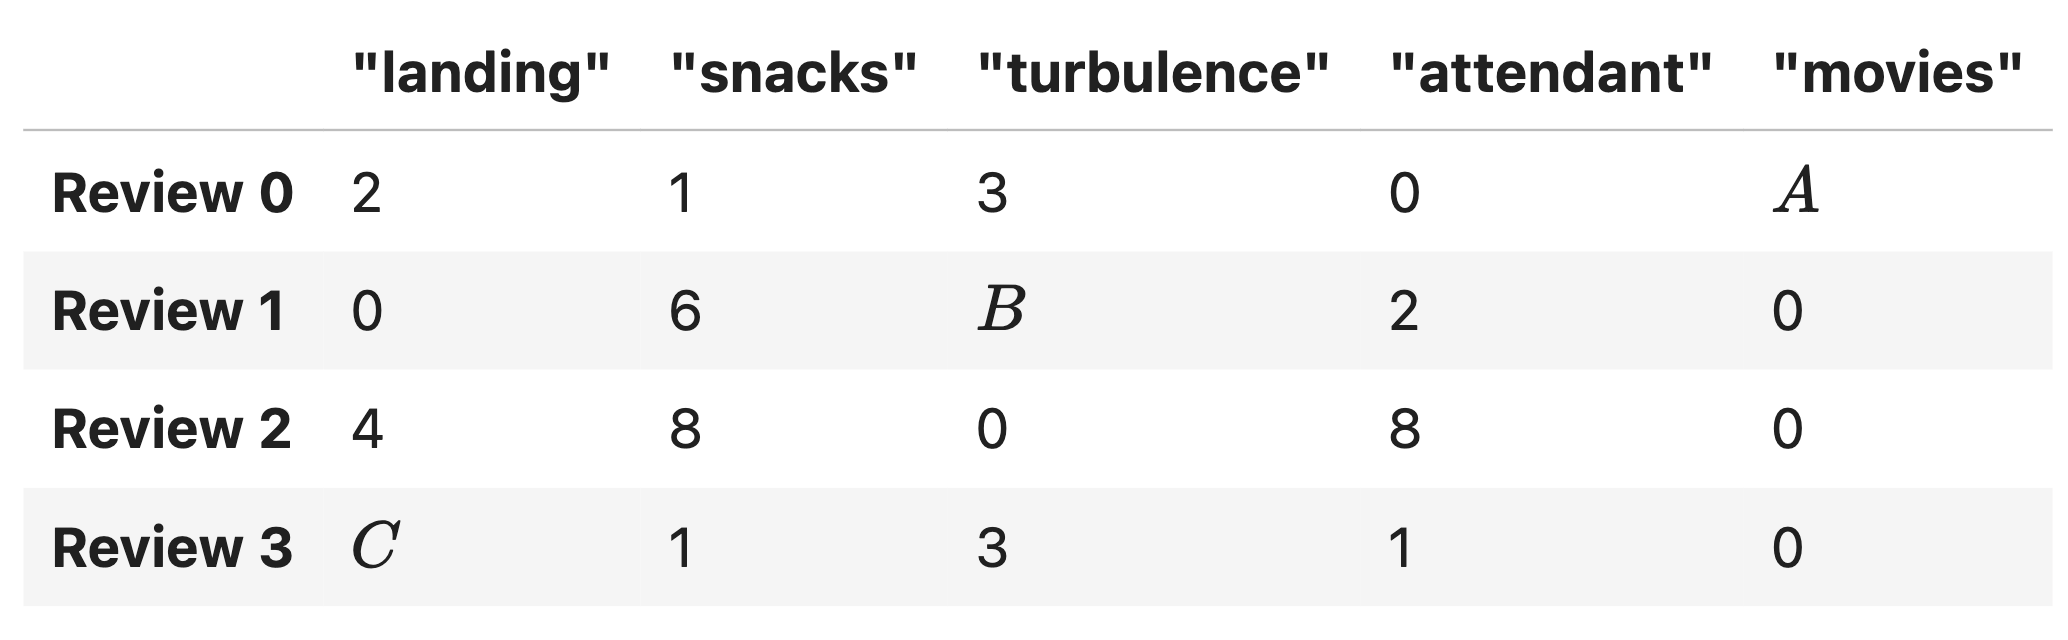
\includegraphics[width=0.8\textwidth]{midterm-images/bow.png}
\end{center}

\vspace{-0.2in}

The matrix has three unknown \textbf{integer} values, $A$, $B$, and $C$. However, we're given that:
\begin{itemize}
    \item The TF-IDF of \texttt{"movies"} in Review 0 is $\frac{5}{4}$.
    \item The TF-IDF of \texttt{"landing"} in Review 2 is $\frac{1}{5}$.
    \item The cosine similarity between the bag of words vectors for Reviews 1 and 2 is $\frac{16}{21}$.
\end{itemize}

\begin{subprobset}

\begin{subprob}(3 pts) What is the value of $A$? Show your work, and $\boxed{\text{box}}$ your final answer.

\begin{responsebox}{1in}
    
\end{responsebox}

\end{subprob}

\begin{subprob}(3 pts) What is the value of $B$? Show your work, and $\boxed{\text{box}}$ your final answer.

\begin{responsebox}{1in}
    
\end{responsebox}

\end{subprob}

\begin{subprob}(3 pts) What is the value of $C$? Show your work, and $\boxed{\text{box}}$ your final answer.

\begin{responsebox}{1in}
    
\end{responsebox}

\end{subprob}
    
\end{subprobset}

% Find the values of $x$, $y$, and $z$ as \textbf{integers}. You can use the empty space to the right for scratch work, but we will not grade any of it.

% \begin{tabular}{ll}
% $x =$ &\inlineresponsebox[1.5in]{} \\
% $y =$ &\inlineresponsebox[1.5in]{} \\
% $z =$ &\inlineresponsebox[1.5in]{}
% \end{tabular}
    
\end{prob}

\newpage

% \begin{prob}

% Suppose \texttt{k} is some positive integer such that:

% \begin{verbatim}
% >>> reviews.iloc[np.arange(-k, k, 3)].shape[0]
% 19
% \end{verbatim}

% What is the value of \texttt{k}?

% \bubble{\texttt{27}} \bubble{\texttt{28}} \bubble{\texttt{29}} \bubble{\texttt{30}} \bubble{\texttt{31}} \bubble{\texttt{32}} \bubble{\texttt{33}}
    
% \end{prob}

\newpage

Make sure you've written your uniqname in the space provided in the top right corner of every page of this exam.

Congrats on finishing the exam! Feel free to draw us a picture about EECS 398 below :)

% (1 pt) And here's a free point!

\begin{responsebox}{7.5in}
    
\end{responsebox}

\end{probset}

\end{document}
